\chapter{Design and Implementation Detail}
\label{design}

\section{Introduction}
\label{des:intro}

In this chapter design and project structure of implemented techniques will be introduced and discussed. Two techniques have been selected to be implemented. This chapter is organized as follows. Section~\ref{des:choose} explains selected techniques and the reasoning behind it. In this section, selected techniques are explained at theoretical level. Section~\ref{des:proj} describes the structure of the implementation for Spark Streaming in detail. Section~\ref{des:conf} describes the configuration parameters required to launch the implementation. Finally, Section~\ref{des:conc} concludes this chapter.

\section{Choosing Auto-Scaling Techniques}
\label{des:choose}

As discussed in Section~\ref{ias:alg-fam}, Auto-Scalers can be categorized into 5 groups.
\begin{description}[leftmargin=0pt]
    \item[Threshold-Based] In this approach, one or multiple threshold values are defined~\cite{Hasan2012IntegratedAA} which specifies the behavior of the Auto-Scaler when the system load goes beyond these thresholds. However, manually defining thresholds is a tricky process~\cite{Dutreilh2010}. Spark's default dynamic resource manager~\cite{spark} and Online Parameter Optimization~\cite{Heinze:2015} are partially based on this approach and they will be evaluated in Section~\ref{eval}.
    \item[Time-Series Analysis] In this approach, a history window of workload -- depending on prediction accuracy -- is considered to predict future workload. However, in case the workload is changing in an unpredictable way -- which is not an unusual phenomena in streaming applications -- then this approach becomes less useful. As confirmed by DEBS grand challenges~\cite{debs2014}~\cite{debs2015}~\cite{debs2016}, the general assumption for streaming applications is that the workload is unpredictable. Due to this limited applicability, no time-series technique is implemented.
    \item[Queuing Theory] In this approach, the system is modeled as a queue network. Since queuing parameters -- message inter-arrival and service rates --  are static, they have to be re-calculated in a timely manner. One of the novel implementations is done by~\textcite{Lohrmann:2015}. However, authors made two unconvincing assumptions. First, worker nodes shall be homogeneous in terms of processing power and network bandwidth. Second, there should be an effective partitioning strategy in place in order to load balance outgoing messages between stages. In reality both assumptions rarely occur. Large scale stream processing clusters are built incrementally. Depending on workload, data skew does exist and imperfect hash functions are widely used by software developers. Furthermore, as confirmed by~\textcite{Rajarshi:2005}, queuing models are very complicated to build and less adaptive to changing environments. As a consequence, no queuing theory technique is implemented.
    \item[Reinforcement Learning] Reinforcement Learning has shown its capabilities to adapt ever changing environments. However, some of the proposed solutions are conflicting with the requirement of this thesis as discussed in Section~\ref{prob-def}. The following summarizes the reasoning why each proposal is accepted or rejected by this thesis.
    \begin{itemize}
        \item \textcite{Herbst:2017} proposed a solution based \emph{Bayesian Networks}. There are two major problems with this proposal. First, it needs sampling and offline training which is inapplicable for changing streaming workloads. Second, in case the model is complex, the training phase is long and computationally infeasible for streaming workloads. As mentioned, both issues are conflicting with thesis requirements.
        \item \textcite{Tesauro2006} proposes a hybrid approach to resolve performance issues of online training which consists of two components. First an online component based on queuing theory. Second, Reinforcement Learning component that is trained offline. This proposal models each node as a queue. However, the only way to apply this technique is to modify \lstinline$spark-core$ package. Thus, this solution is not implemented.
        \item \textcite{Rao:2009:VRL} proposed a solution to manage virtual machine resources. However, it is also based on offline training and sampling which is obtained from a separate supervised training phase. Thus, it's not applicable for dynamic streaming workloads. 
        \item \textcite{Enda:2012} proposed a parallel architecture to Reinforcement Learning without any global controller involved. Nodes (RL agents) have two tables. Local table is trained by each node separately. Global table contains values learned by other nodes. When an agent learns anything new, it broadcasts it to other nodes. From theoretical point of view, this solution might seem feasible, since parallel learning speeds up initialization process. However, Spark has a single global controller. Applying this technique to Spark requires heavy modification to \lstinline$spark-core$ package. 
        \item \textcite{Heinze:2014} implemented Reinforcement Learning in the context of FUGU~\cite{Grandl:2014:MPC}. Each node, maintains its own Q-Table and imposes local policy without coordinating with other nodes. Although this architecture is not applicable for Spark, but its core idea -- \emph{Temporal Difference}~\cite{rlIntro} algorithm-- is applicable. Thus, this thesis implemented this proposal by adopting it to Spark architecture. Refer to Section~\ref{des:temp} for theoretical background and Section~\ref{des:proj} for implementation detail.
        \item \textcite{CARDELLINI2018171} proposed a two level hierarchical architecture for resource management in Apache Storm~\cite{Storm}. Local controller applies local policy on each node and coordinates with the global controller for confirmation of its actions. Although, this architecture seems to be a promising approach, however it has been implemented by modifying Storm's internal components. As mentioned above, this is in conflict with thesis's requirements.
        \item \textcite{dutreilh:hal-01122123} proposed a model-based Reinforcement Learning approach for resource management which is based on a global controller. In order to overcome the slow convergence of model-free learning, authors proposed to estimate environment dynamics based on collected samples at runtime. Then it switches to \emph{Value Iteration}~\cite{rlIntro} algorithm instead of \emph{Temporal Difference}. This approach has also been partially adopted by this thesis. Refer to Section~\ref{des:val} for theoretical background and Section~\ref{des:proj} for implementation detail.
    \end{itemize}
    \item[Control Theory] Techniques based on Control Theory are also promising for elastic data streaming. Because it monitors input and output of the application, it can respond to workload changes very fast and adapt the system if necessary. Thus it is perfectly capable of handling dynamic environments. The comparison between Reinforcement Learning and Control Theory techniques is left for future work.
\end{description}
As mentioned, two techniques -- \emph{Temporal Difference} and \emph{Value Iteration} -- will be implemented in this thesis. In next two sections, theoretical foundation of these algorithms will be laid out. Noteworthy to mention, these sections are heavily inspired by~\textcite{rlIntro}. Furthermore, Section~\ref{related} discusses more techniques and the reasoning why they have been rejected by this thesis.
\clearpage
\subsection{Temporal Difference}
\label{des:temp}
Section~\ref{ias:alg-rl} explains the basics of Reinforcement Learning. Temporal Difference (TD) learning is one of the foundational algorithms of Reinforcement Learning. It can learn from applying experience without having prior knowledge about environment's dynamics. This property is potentially useful for data stream processing systems in which the incoming workload is changing without any particular pattern.

Before starting to dig into details, some formal notions shall to be explained. An \emph{episode} is series of experiences that is taken by the agent. At each time step~$t$, the agent moves from one \emph{state}~$S_t$ to another state~$S_{t+1}$. A \emph{policy} $\pi$ defines the action~$A_t$ that should be taken by the agent at each state. Followed by each action, the agent receives a \emph{reward}~$R_{t+1}$ from the environment. Note that, the agent will receive reward for its corresponding action at next state~$S_{t+1}$. Thus, an episode can be viewed as Equation~\ref{des:eq:episode}.
\begin{equation}
\dots\,S_t,\,A_t,\,R_{t+1},\,S_{t+1},\,A_{t+1},\,R_{t+2},\,S_{t+2},\,A_{t+2},\,R_{t+3}\,\dots
\label{des:eq:episode}
\end{equation}

An episode does not necessarily have a \emph{terminal} state. In some environments -- like data stream processing -- an episode is a never ending sequence of experiences. Prior to taking an action, the agent has an estimate of \emph{expected reward}~$V$ which specifies future reward if it follows the same actions returned by policy~$\pi$ from that specific state. Thus, it is referred as $V_\pi$ which translates to expected future reward under policy~$\pi$. During the episode, the agent tries to \emph{maximize} the reward that it received from the environment. Any policy that leads to maximum possible reward is called the \emph{optimal} policy~$\pi^*$ and its corresponding estimate of future reward is referred to as~$V^{*}_{\pi}$.

Unlike Monte Carlo~\cite{rlIntro} methods that requires agent to wait until the end of episode, TD approaches only need to wait until the end of next time step to get a feedback from environment. Then, the agent updates corresponding estimate of previous state. Thus, the most simple TD approach can be formulated as Equation~\ref{des:eq:std}. Equation~\ref{des:eq:std} contains two important parameters of TD.
\begin{equation}
V(S_t) \longleftarrow (1-\alpha)V(S_t) + \alpha\big[R_{t+1} + \gamma\,V(S_{t+1})\big]
\label{des:eq:std}
\end{equation}
\begin{itemize}
	\item $\bm{\alpha}$ denotes \emph{Learning Factor}. It specifies, how much the agent shall learn from new experiences. A higher $\alpha$ means learning with a faster pace. It also leads to forgetting history faster. On the other hand, a lower $\alpha$ leads to slower learning process which means the agent trusts its experience history more -- it gives more weight to history rather than new experiences. $\alpha$ is defined as a number between (0,1].
	\item $\bm{\gamma}$ denotes \emph{Reward Factor} or \emph{Discount Factor}. It specifies, whether the agent shall optimize for \emph{future} or \emph{immediate} reward. A higher $\gamma$ leads to optimizing for future reward, whereas a lower $\gamma$ leads to optimizing for immediate reward. It is defined as a number between (0,1). As defined by Equation~\ref{des:eq:reward}, reward is cumulating at each time step which causes the sum to grow indefinitely. In order to prevent infinite reward problem, it is crucial to define $\gamma$ as a number less than one to force convergence.
	\begin{equation}
	R_t = r_{t+1}+\gamma r_{t+2}+\gamma^2 r_{t+3}+\dots=\sum_{0}^{\infty}\gamma^k r_{t+k+1}
	\label{des:eq:reward}
	\end{equation}
\end{itemize}

Since expected future reward is defined per action, Equation~\ref{des:eq:std} changes slightly and becomes as Equation~\ref{des:eq:qtd}. This update is applied after every transition from a nonterminal state $S_t$. In case $S_{t+1}$ is terminal, then $Q(S_{t+1},\,A_{t+1})$ is set to zero. As a consequence, each experiment can be defined with a quadruple of (State, Action, Reward, State$'$) or $(S_{t},\,A_{t},\,R_{t+1},\,S_{t+1})$. This method is known as \emph{Sarsa} algorithm and named \emph{Q-Learning} because of the Q-Table used in the equation. Algorithm~\ref{des:a:ql}\footnote{The pseudocode has been taken from~\textcite{rlIntro}} describes this procedure.
\begin{equation}
Q(S_t,\,A_t) \longleftarrow (1-\alpha)Q(S_t,\,A_t) + \alpha\big[R_{t+1} + \gamma\,Q(S_{t+1},\,A_{t+1})\big]
\label{des:eq:qtd}
\end{equation}
\begin{algorithm}[t]
	\DontPrintSemicolon
	
	Algorithm parameters: $\alpha \in (0,1]$, $\gamma \in (0,1)$\;
	Initialize $Q(s,\,a)$ for all $s \in \{S - terminal\}$, $a \in A(s)$ arbitrarily and $Q(terminal,a) = 0$\;
	\BlankLine
	\Repeat{\text{End of episode or $S$ is terminal}} {
		Take action $A$ based on policy $\pi$ derived from $Q$ table\;
		Observe reward $R$ and land in state $S'$\;
		Choose $A'$ from $S'$ using the same policy $\pi$\;
		$Q(S,\,A) \gets (1-\alpha)\;Q(S,\,A) + \alpha\;\big[R + \gamma\;Q(S',\,A')\big]$\;
		$S \gets S'$\;
		$A \gets A'$\;
	}
	\caption{Q-Learning Work-Flow}
	\label{des:a:ql}
\end{algorithm}

An agent takes action based on a policy function~$\pi$ which in turn is derived -- partially or completely -- from the Q-Table. However, it shall be noted that in the beginning of episode the Q-Table is initialized to zero. In such situations, it takes very long time for agent to discover new states which is particularly harmful for data stream processing systems. This problem is usually solved by introducing small degree of randomness. The policy function decides randomly with a small probability~$\epsilon$ and in any other case~($1-\epsilon$), it behaves based on Q-Table. Other solutions do exist to solve state discovery problem. For example, Q-Table can be initialized with a random value or based on some \emph{heuristic} function that is partially derived from domain knowledge. 

Furthermore, if two or more actions have equal expected reward, then policy function has to decide on one of them by breaking the tie. There are different strategies to solve this issue. Choosing a random action is one of them. However, in some domains this might be dangerous or harmful. Rather than choosing randomly, a simple heuristic inspired by domain knowledge can be helpful too.
\subsection{Value Iteration}
\label{des:val}

As mentioned in last section, in streaming workloads the common belief is that the workload is not predictable. In other words, reward values of each action and probability of landing in a specific state after taking an action -- environment dynamics -- is unknown. However for the sake of discussion, let us assume environment dynamics is \emph{known}. In such situations, Reinforcement Learning can be solved using \emph{Dynamic Programming} techniques. In this section, the problem will be solved for environments with known dynamics. Then, some of the core ideas will be applied to adopt the solution for environments with unknown dynamics.

Finding an optimal policy function, when environments dynamics is known can be \emph{recursively} solved by applying dynamic programming. As mentioned previously, the agent is trying to maximize expected reward by taking optimal actions. Here expected reward is defined with $\mathbb E$ and $\underset{a}{\text{max}}$ selects maximum value based on specified action.

\begin{equation}
\begin{aligned}[h]
V^*(s) &= \underset{a}{\text{max}} \; \mathbb E\;\big[R_{t+1} + \gamma\:V^*(S_{t+1})\,|\,S_t=s,\,A_t=a\big] \\
&= \underset{a}{\text{max}} \; \sum_{s',r} p(s',r\,|\,s,a)\;\Big[r + \gamma\:V^*(s')\Big]
\end{aligned}
\label{des:eq:dpv}
\end{equation}
\begin{equation}
\begin{aligned}[h]
Q^*(s,a) &= \mathbb E\;\big[R_{t+1} + \gamma\:\underset{a'}{\text{max}}\;Q^*(S_{t+1},a')\,|\,S_t=s,\,A_t=a\big] \\
&= \sum_{s',r} p(s',r\,|\,s,a)\;\Big[r + \gamma\:\underset{a'}{\text{max}}\;Q^*(S_{t+1},a')\Big]
\end{aligned}
\label{des:eq:dpq}
\end{equation}

For scenarios where $p$ and $r$ are unknown -- which is the case for this thesis -- these values can estimated by collecting samples. As the agent runs for some period of time, it collects samples and then estimates $p$ and $r$. Given that $p$ and $r$ are estimated to some degree, it is possible to initialize Q-Table with more useful values -- compared to zero or random values -- and speed up learning process. Whether this estimation is accurate or not -- how many samples shall be collected for a precise estimation -- is another question which will be evaluated in Section~\ref{eval}.

The following procedure is applied for collecting samples which is inspired by \textcite{dutreilh:hal-01122123}. As agent runs and observes a quadruple of ($s,a,r,s'$), the following counters are updated.
\begin{equation}
\begin{aligned}[h]
P[s,a,s'] &= P[s,a,s'] + 1\\
R[s,a] &= R[s,a] + r \\
C[s,a] &= C[s,a] + 1
\end{aligned}
\end{equation}
Given these statistics, estimators $\overline{P}$, $\overline{R}$ are calculated to replace original $p$, $r$ in Equation~\ref{des:eq:dpq} respectively.
\begin{equation}
\begin{aligned}[h]
\overline{P}[s,a,s'] &= \frac{P[s,a,s']}{C[s,a]} \\
\overline{R}[s,a] &= \frac{R[s,a]}{C[s,a]}
\end{aligned}
\end{equation}

After estimating $p$, $r$, Algorithm~\ref{des:a:vi}\footnote{The pseudocode has been taken from~\textcite{rlIntro}} can be used to produce optimal policy. Not the difference between \textbf{max} and \textbf{argmax} functions. The former returns the \emph{maximum value} and the later returns the \emph{action that has the maximum value}. Value Iteration that described in Algorithm~\ref{des:a:vi} can be used independent of Temporal Difference. However, in this thesis it is used to get a useful initialized Q-Table. Thus, when sample collection period is over and Q-Table is initialized, normal Q-Learning approach is used thereafter. The reason is that in Value Iteration, after sampling period, Q-Table is never updated again. However, by combining Value Iteration -- for initializing Q-Table -- and Q-Learning, Q-Table is also updated at runtime which improves decision accuracy.
\begin{algorithm}[h]
	\DontPrintSemicolon
	
	A small threshold $\theta > 0$ determining accuracy of estimation\;
	Initialize $V(s)$ for all $s \in \{S - terminal\}$ arbitrarily and $V(terminal) = 0$\;
	\BlankLine
	\Repeat{$\Delta < \theta$} {
		$\Delta \gets 0$\;
		\ForEach{$s \in S$}{
			$v \gets V(s)$\;
			$V(s) \gets \text{max}_a\;\sum_{s',r} p(s',r\,|\,s,a)\;\Big[r + \gamma\:V(s')\Big]$ \;
			$\Delta \gets \text{max}(\Delta,|v - V(s)|)$
		}
		\BlankLine
		Output policy $\pi \approx \pi^*$, such that\;
		$\pi(s) = \text{argmax}_a\;\sum_{s',r} p(s',r\,|\,s,a)\;\Big[r + \gamma\:V(s')\Big]$
	}
	\caption{Value Iteration for Estimating $\pi \approx \pi^*$}
	\label{des:a:vi}
\end{algorithm}

\clearpage
\section{Design}
\label{des:proj}

In this section technical design and structure of the thesis will be explained and discussed. As mentioned in previous section, two Reinforcement Learning techniques -- namely Q-Learning (Temporal Difference) and Value Iteration -- have been implemented. Both of these methods require defining \emph{state space}, \emph{policy} and \emph{reward} functions. Typically, Reinforcement Learning agents move from one state to another by taking an action which is proposed by policy function, getting feedback -- known as reward -- from environment and landing into destination state. In next sections each of these components will be discussed.

\subsection{State Space}
\label{des:state-space}

State space defines -- models -- the environment where the agent is living. Usually, it is combination of environment's properties. The following is list of sample state spaces that could be defined for different applications.
\begin{description}[leftmargin=0pt]
    \item[Web Applications] For a typical web application, a sample state space could be defined as a tuple of
    \begin{center}
        [Number of web servers, Total workload defined as requests per second, Average round trip delay of requests]
    \end{center}
    \item[Virtualization Server] For a Hypervisor, a sample state space can be defined as a tuple of
    \begin{center}
        [Number of running virtual machines, Total CPU utilization, Total used RAM]
    \end{center}
    \item[Stream Processing] For a data stream processing system, a sample state space can be defined as a tuple of
    \begin{center}
        [Number of worker nodes, Total workload defined as messages per second, Average latency of messages]
    \end{center}
\end{description}
As state space contains more precise information, it gets bigger and bigger. Thus, in most systems it is \emph{discretized} to some degree to reduce its size. State space reduction has a couple of benefits.
\begin{itemize}
    \item \textbf{Change Observation}. For example, in most systems a 1\% increase/decrease in CPU utilization is not considered as a noticeable change but 5\% is.
    \item \textbf{Absorbing Sudden Bursts}. In some applications, there might be a sudden change in one aspect of the system for a slightly short time. For example 20\% increase in CPU utilization for 5 seconds may not be considered as sustained workload increase.
    \item \textbf{Preventing Zig-Zag Decisions}. If state space is discretized to fine-grained states, it might lead to consecutive contradictory decisions -- A phenomena known as \emph{Zig-Zag} decisions. For example, Auto-Scaler may decide to perform a scale-in action in one step and scale-out action in next step. A reasonable way to prevent this never ending loop is to discretize the state space into coarse-grained states.
\end{itemize}
However, it shall be noted that \emph{over discretizing} the state space may have negative impacts on target system. Section~\ref{eval} contains an experiment to evaluate discretization impact.

In this thesis, a combination of latency and direction of workload is incorporated in to state space.
\begin{description}[leftmargin=0pt]
    \item[Latency] Each micro-batch is associated with two latencies. First, \emph{Processing Latency} -- time that takes to process a single micro-batch from start to end. second, \emph{Scheduling Latency} -- time that each micro-batch stays in a queue \emph{waiting} to be processed. In this project, total latency (processing latency + scheduling latency) is stored as an average value calculated over a window of time.
    \item[Workload Direction] It is reasonable to consider average number of messages that are being processed in state space. However, in order to reduce state space only its \emph{direction} is stored. That is, instead of storing a pure number as average number of messages processed per window of time, only a boolean value indicating that incoming messages are increased to decreased -- compared to last window -- is stored.
\end{description}

As mentioned in Section~\ref{intro-auto-scale} each state is associated with three actions -- No-Action, Scale-In and Scale-Out. Each action has corresponding reward -- Q-Value-- attached to it. Figure~\ref{des:l:state-space} depicts this relationship.
\begin{figure}[h]
    \centering
    \begin{tikzpicture}[show background grid]
    \begin{class}[text width=10cm]{StateSpace}{7,0}
        \attribute{- stateToActionSet: HashMap<State, HashMap<Action, Double>{}>}
        \operation{+ addState(s: State)}
        \operation{+ size()}
        \operation{+ updateQValueForAction(s: State, a: Action, qValue: Double)}
    \end{class}
    \begin{class}{State}{12,-5}
        \attribute{+ latency: Integer}
        \attribute{+ isLoadIncreasing: Boolean}
    \end{class}
    \begin{interface}{Action}{4,-5}
        \operation[0]{+ toString()}
    \end{interface}
    \begin{class}[text width=3cm]{NoAction}{0,-8}
        \implement{Action}
        \operation{+ toString()}
    \end{class}
    \begin{class}[text width=3cm]{ScaleIn}{4,-8}
        \implement{Action}
        \operation{+ toString()}
    \end{class}
    \begin{class}[text width=3cm]{ScaleOut}{8,-8}
        \implement{Action}
        \operation{+ toString()}
    \end{class}
    
    \aggregation{StateSpace}{}{}{State}
    \aggregation{StateSpace}{}{}{Action}
    
    \path (StateSpace) -- (State) node[midway,sloped,above]{states}
    node[midway,sloped,below] {1..*};
    \path (StateSpace) -- (Action) node[midway,sloped,above]{actionSet}
    node[midway,sloped,below] {1..*};
    \end{tikzpicture}
    \caption{State Space Class Diagram}
    \label{des:l:state-space}
\end{figure}

\subsection{State Space Initialization}
\label{des:state-init}

Typically when the agent starts, its Q-Table is empty -- initialized with zero. Over time, as the agent take more actions and discovers its environment, it updates its Q-Table. Since Q-Table is initialized with zero, the agent usually takes some random actions from time to time with a small probability.This helps to discover the environment. In some applications, this behavior is sufficient. However, in fast changing environments like streaming systems this process takes very long time to converge. Thus developers usually try to initialize Q-Table beforehand to speedup the learning process. In this thesis, three different initializers have been implemented. Figure~\ref{des:f:ss-init} shows class diagram of these initializers.
\begin{description}[leftmargin=0pt]
\item[Zero Initializer] This is the default implementation which initializes all the Q-Values -- reward values -- to zero.
\item[Random Initializer] This initializer assigns a random value between (-1,1) to Q-Values.
\item[Optimized Initializer] This initializer uses a \emph{heuristic} to initialize the Q-Table. Typically in most systems, there is a well defined set of SLOs defined by users that should be respected by Auto-Scaling system. This initializer exploits a normalization function defined in Equation~\ref{des:eq:normal}. If recent latency window is sufficiently large enough, workload-to-latency graph looks similar to Figure~\ref{des:f:ss-region}. This graph is divided into four regions. As workload increases, latency is approaching target latency (Region 1). In case the workload keeps increasing, the agent goes beyond the target latency and SLOs are violated (Region 2). Assuming the agent takes some reasonable action, latency starts to decrease (Region 3). Finally, at some point it will drop below the target latency line (Region 4). For each region, Q-Table is initialized with different values.
\begin{equation}
n = \frac{\text{current latency}}{\text{target latency}}
\label{des:eq:normal}
\end{equation}
\end{description}
\begin{figure}[t]
    \centering
    \begin{tikzpicture}[show background grid]
    \begin{interface}{StateSpaceInitializer}{5,0}
        \operation{+ getInstance()}
        \operation[0]{+ initialize(ss: StateSpace)}
    \end{interface}
    \begin{class}[text width=5cm]{ZeroStateSpaceInitializer}{0,-4}
        \implement{StateSpaceInitializer}
        \operation{+ initialize(ss: StateSpace)}
    \end{class}
    \begin{class}[text width=5cm]{RandomStateSpaceInitializer}{5,-6}
        \implement{StateSpaceInitializer}
        \operation{+ initialize(ss: StateSpace)}
    \end{class}
    \begin{class}[text width=5cm]{OptimizedStateSpaceInitializer}{10,-4}
        \implement{StateSpaceInitializer}
        \operation{+ initialize(ss: StateSpace)}
    \end{class}
    \end{tikzpicture}
    \caption{State Space Initializer}
    \label{des:f:ss-init}
\end{figure}
\begin{figure}[h]
    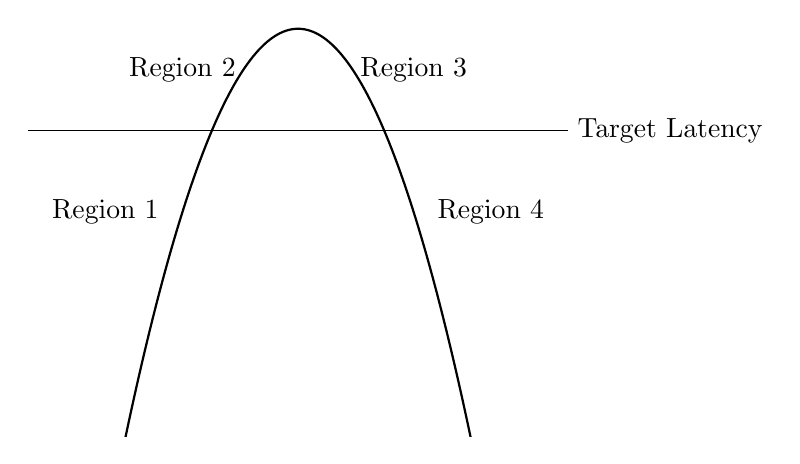
\begin{tikzpicture}
        \begin{axis}[
            ticks=none,
            axis x line=center,
            x axis line style=-,
            hide y axis,
            xlabel style={right},
            samples = 200,
            domain = -7:7,
            xmin = -7, xmax = 7,
            ymin = -15, ymax = 7,
            xlabel={Target Latency}]
            \addplot[black, thick, mark=none] {-x^2 + 5};
            \node[] at (axis cs: -5,-4) {Region 1};
            \node[] at (axis cs: -3,3) {Region 2};
            \node[] at (axis cs: 3,3) {Region 3};
            \node[] at (axis cs: 5,-4) {Region 4};
        \end{axis}
    \end{tikzpicture}
    \centering
    \caption{Different Regions of a Typical Workload}
    \label{des:f:ss-region}
\end{figure}
\clearpage
The following describes the way all four regions are initialized. Table~\ref{des:tab:rules} summarizes each region and describes preferred action in each region.
\begin{description}[leftmargin=0pt]
    \item[Region 1] In this region, latency is increasing as workload is increasing. So it is reasonable to give more reward to Scale-Out as the agent approaches target latency line. This is called \emph{Early Scale-Out} action which helps to add worker tasks in order to prevent violating SLOs. Thus the reward for each action is initialized as Equation~\ref{des:eq:r1}. In this region, Scale-Out and NoAction rewards are positive but less than one.
    \begin{equation}
    \text{Scale-Out}=\frac{\text{current latency}}{\text{target latency}} \qquad \text{NoAction}=1-\frac{\text{current latency}}{\text{target latency}} \qquad \text{ScaleIn}=0
    \label{des:eq:r1}
    \end{equation}
    \item[Region 2] In this region, the agent has fall behind and latency has been increased up to the point that it is more than target latency. At this point Scale-Out is still the preferred action. It is reasonable to initialize Scale-In with a negative reward to prevent the agent from taking unjustifiable action.
    Reward for each action is initialized as Equation~\ref{des:eq:r2}. In this region, Scale-Out reward is larger than one but NoAction reward is less than one.
    \begin{equation}
    \text{Scale-Out}=\frac{\text{current latency}}{\text{target latency}} \qquad \text{NoAction}=\frac{\text{current latency}}{\text{target latency}}-1 \qquad \text{ScaleIn}=-1
    \label{des:eq:r2}
    \end{equation}
    \item[Region 3] In this region, either the workload is decreasing or the agent has taken a presumably reasonable action that has led latency to decrease. Usually, it is not required to take any further action here. Thus, to let latency stabilize, NoAction is a preferred action in this region. Additionally, Scale-In is still prohibited.
    \begin{equation}
    \text{Scale-Out}=0 \qquad \text{NoAction}=1 \qquad \text{ScaleIn}=-1
    \label{des:eq:r3}
    \end{equation}
    \item[Region 4] In this region, the latency has dropped below target latency and is decreasing gradually. Thus, as the agent gets farther away from target latency line, we encourage the agent to take Scale-In action. However, near target latency line, we still prefer to take NoAction, since it is still dangerous to take Scale-In.
    \begin{equation}
    \text{Scale-Out}=0 \qquad \text{NoAction}=\frac{\text{current latency}}{\text{target latency}} \qquad \text{ScaleIn}=1-\frac{\text{current latency}}{\text{target latency}}
    \label{des:eq:r4}
    \end{equation}
\end{description}
\begin{table*}[h]
    \begin{tabular}{ll}
        \toprule
        \textbf{Region} & \textbf{Preferred Behavior}\\
        \midrule
        Region 1 & Early Scale-Out is preferred to avoid hitting target latency.\\
        Region 2 & Target latency is already violated, so Scale-Out is still preferred.\\
        Region 3 & Although latency is higher than target -- but decreasing, NoAction is preferred to let latency stabilize.\\
        Region 4 & Latency is stable again. If latency is sufficiently low, then Scale-In is preferred.\\
        \bottomrule
    \end{tabular}
    \centering
    \caption{Summary of Latency Regions}
    \label{des:tab:rules}
\end{table*}

\clearpage
\subsection{Policy Functions}
\label{des:pol}

Policy $\pi$ is a function that guides the agent to take an action in each state. Different strategies can be implemented but at its core, a policy function is either extracted from Q-Table. An optimal policy $\pi^*$ is a policy that returns actions that lead to maximum expected reward. Before getting into details about implemented policies of this thesis, \emph{monotonicity constraint}~\cite{Herodotou:2011} shall be explained. Monotonicity constraint mandates:
\begin{itemize}
    \item If Scale-Out was the chosen action in last state and latency has been increased -- compared to last state, then it is not possible to take Scale-In in current state. The reason is that, even by applying Scale-Out, latency has been increased. So, for a even higher latency, there is no reason that Scale-In could ever help.
    \item If Scale-In was the chosen action in last state and latency has been decreased -- compared to last state, then it is not possible to take Scale-Out in current state. The reason is that, latency is decreasing without taking Scale-Out. So, for a even lower latency, there is no need for Scale-Out. Even though Scale-Out is a safe action in this case, but in Spark Streaming any Scale-In/Out action cause reshuffling of intermediate results. Thus, it is crucial to avoid unnecessary -- although safe -- actions.
\end{itemize}
As confirmed by~\textcite{Heinze:2014}, monotonicity constraint improves learning process. Algorithm~\ref{des:a:mono} shows the pseudocode of this procedure.
\begin{algorithm}[h]
    \DontPrintSemicolon
    \SetKwData{cs}{currentState}
    \SetKwData{ls}{lastState}
    \SetKwData{la}{lastAction}
    \SetKwArray{ca}{feasibleActions}
    \ca $\gets$ GetActionsFromStateSpace(\cs)\;
    \BlankLine
    \If{\cs.latency > \ls.latency AND \la == ScaleOut}{
        \ca $\gets \ca\;-\;$ScaleIn
    }
    \BlankLine
    \If{\cs.latency < \ls.latency AND \la == ScaleIn}{
        \ca $\gets \ca\;-\;$ScaleOut
    }
    \caption{Monotonicity Constraint}
    \label{des:a:mono}
\end{algorithm}


Three different policies have been implemented in this thesis. Figure~\ref{des:f:policy} depicts class diagram of these polices. Table~\ref{des:tab:policy} summarizes the behavior of each policy.
\begin{description}[leftmargin=0pt]
    \item[Greedy Policy] This policy takes action in two phases. First, it applies monotonicity property. After that, it selects the best possible action. Best action here means the action with largest/lowest Q-Value, depending on how reward function has been implemented.
    \item[One Minus Epsilon Policy] This policy wrap any other policy and adds some degree of randomness to it. That is, with a probability of $\epsilon$ it returns a random action and with a probability of $1-\epsilon$ it hands over the process to underlying policy. Underlying policy is not necessarily an optimal -- greedy -- policy.
    \item[Decreasing One Minus Epsilon Policy] This policy is similar to previous policy. The different is that randomness~($\epsilon$) is decreasing over time until it reaches zero after which it unconditionally hands over to underlying policy.
\end{description}
\begin{table*}[h]
    \begin{tabular}{ll}
        \toprule
        \textbf{Policy} & \textbf{Behavior}\\
        \midrule
        Greedy & Always stick to action with highest/lowest Q-Value.\\
        One Minus Epsilon & Take random action with a probability of $\epsilon$, otherwise stick to underlying policy. \\
        Decreasing One Minus Epsilon & Same as $1-\epsilon$ policy, but $\epsilon$ is decreasing over time.\\
        \bottomrule
    \end{tabular}
    \centering
    \caption{Summary of Policy Functions}
    \label{des:tab:policy}
\end{table*}
\begin{figure}[h]
    \centering
    \begin{tikzpicture}[show background grid]
    \begin{interface}{Policy}{4,0}
    \operation[0]{+ nextAction(currentState: State)}
    \end{interface}
    \begin{class}[text width=6cm]{GreedyPolicy}{0,-4}
    \implement{Policy}
    \operation{+ nextAction(currentState: State)}
    \end{class}
    \begin{class}[text width=6cm]{OneMinusEpsilonPolicy}{8,-4}
    \implement{Policy}
    \attribute{- underlyingPolicy: Policy}
    \attribute{- epsilon: Double}
    \operation{+ nextAction(currentState: State)}
    \end{class}
    \begin{class}[text width=6cm]{DecreasingOneMinusEpsilonPolicy}{8,-8}
    \inherit{OneMinusEpsilonPolicy}
    \attribute{- epsilon: Double}
    \operation{+ nextAction(currentState: State)}
    \end{class}
    \end{tikzpicture}
    \caption{Policy Functions}
    \label{des:f:policy}
\end{figure}

\subsection{Reward Function}

\clearpage
\section{Configuration}
\label{des:conf}

\section{Conclusion}
\label{des:conc}